% !TEX root = ../sommaire.tex

\chapter{Attribute Inference Attacks for Federated Regression Tasks}

% %%%%%%%%%%%%%%%%%%%%%%%%%%%%%
% \section{Équation}
% %%%%%%%%%%%%%%%%%%%%%%%%%%%%%

%   $$
%   \begin{array}{l c l}
%     Z = \min c\cdotp x & & Z_{LR}(\lambda) = \min c\cdotp x + \lambda^T\cdotp(b_h - A_hx)\\
%     \mbox{s.t. }
%       \left\{
%         \begin{array}{l}
%           A_hx \geq b_h\\
%           A_ex \geq b_e\\
%           x \in \{0, 1\}
%         \end{array}
%       \right.
%     & \longrightarrow
%     & \mbox{s.t. }
%       \left\{
%         \begin{array}{l}
%           A_ex \geq b_e\\
%           x \in \{0, 1\}
%         \end{array}
%       \right.
%   \end{array}
%   $$
  
  
% \begin{figure}
%   \caption{Figure vide}
% \end{figure}


% %%%%%%%%%%%%%%%%%%%%%%%%%%%%%
% \section{Cosinus}
% %%%%%%%%%%%%%%%%%%%%%%%%%%%%%

% \def\b#1{\textcolor{bleu}{#1}}
% \def\V#1{\textcolor{violet}{#1}}
% \def\r#1{\textcolor{pink}{#1}}
% \def\o#1{\textcolor{orange}{#1}}
% \def\g#1{\textcolor{vert}{#1}}

% \begin{figure}
%   \begin{tikzpicture}
%     \draw[->, black!50] (0, -1.5) -- (0, 1.5);
%     \draw[->, black!50] (-1.5, 0) -- (1.5, 0);
%     \begin{scope}[thick, bleu]
%       \clip (0, 0) rectangle (1.5, 1.5);
%       \draw (0, 0) circle (1);
%       \draw (0.5, 0.5) node {1};
%     \end{scope}
%     \begin{scope}[thick, pink]
%       \clip (0, 0) rectangle (-1.5, 1.5);
%       \draw (0, 0) circle (1);
%       \draw (-0.5, 0.5) node {2};
%     \end{scope}
%     \begin{scope}[thick, violet]
%       \clip (0, 0) rectangle (-1.5, -1.5);
%       \draw (0, 0) circle (1);
%       \draw (-0.5, -0.5) node {3};
%     \end{scope}
%     \begin{scope}[thick, orange]
%       \clip (0, 0) rectangle (1.5, -1.5);
%       \draw (0, 0) circle (1);
%       \draw (0.5, -0.5) node {4};
%     \end{scope}
%   \end{tikzpicture}
%   \begin{tikzpicture}[xscale = 1.25]
%     \draw[->, black!50] (0, -1.5) -- (0, 1.5);
%     \draw[->, black!50] (-0.5, 0) -- (8.5, 0);
%     \draw[dotted] (1, -1.5) -- (1, 1.5);
%     \draw[dotted] (2, -1.5) -- (2, 1.5);
%     \draw[dotted] (3, -1.5) -- (3, 1.5);
%     \draw[dotted] (4, -1.5) -- (4, 1.5);
%     \draw[dotted] (5, -1.5) -- (5, 1.5);
%     \draw[dotted] (6, -1.5) -- (6, 1.5);
%     \draw[dotted] (7, -1.5) -- (7, 1.5);
%     \begin{scope}[thick, bleu]
%       \clip (0, 1.5) rectangle (1, -1.5);
%       \draw (0, 1) cos (1, 0) sin (2, -1) cos (3, 0) sin (4, 1);
%       \draw (0.5, 0) node {1};
%     \end{scope}
%     \begin{scope}[thick, pink]
%       \clip (1, 1.5) rectangle (2, -1.5);
%       \draw (0, 1) cos (1, 0) sin (2, -1) cos (3, 0) sin (4, 1);
%       \draw (1.5, 0) node {2};
%     \end{scope}
%     \begin{scope}[thick, violet]
%       \clip (2, 1.5) rectangle (3, -1.5);
%       \draw (0, 1) cos (1, 0) sin (2, -1) cos (3, 0) sin (4, 1);
%       \draw (2.5, 0) node {3};
%     \end{scope}
%     \begin{scope}[thick, orange]
%       \clip (3, 1.5) rectangle (4, -1.5);
%       \draw (0, 1) cos (1, 0) sin (2, -1) cos (3, 0) sin (4, 1);
%       \draw (3.5, 0) node {4};
%     \end{scope}
    
%     \begin{scope}[xshift = 4cm]
%     \begin{scope}[thick, bleu]
%       \clip (0, 1.5) rectangle (1, -1.5);
%       \draw (0, 1) cos (1, 0) sin (2, -1) cos (3, 0) sin (4, 1);
%       \draw (0.5, 0) node {1};
%     \end{scope}
%     \begin{scope}[thick, pink]
%       \clip (1, 1.5) rectangle (2, -1.5);
%       \draw (0, 1) cos (1, 0) sin (2, -1) cos (3, 0) sin (4, 1);
%       \draw (1.5, 0) node {2};
%     \end{scope}
%     \begin{scope}[thick, violet]
%       \clip (2, 1.5) rectangle (3, -1.5);
%       \draw (0, 1) cos (1, 0) sin (2, -1) cos (3, 0) sin (4, 1);
%       \draw (2.5, 0) node {3};
%     \end{scope}
%     \begin{scope}[thick, orange]
%       \clip (3, 1.5) rectangle (4, -1.5);
%       \draw (0, 1) cos (1, 0) sin (2, -1) cos (3, 0) sin (4, 1);
%       \draw (3.5, 0) node {4};
%     \end{scope}
%     \end{scope}
%   \end{tikzpicture}
%   \caption{Cosinus}
% \end{figure}
  
  
%   $\cos([x^-, x^+]) = [-1, 1]$ si $x^+ - x^- \geq 2\pi$
  
%   sinon
  
%   $\begin{array}{c | c | l}
%   x^- \mod 2\pi \in & x^+ \mod 2\pi \in & \cos([x^-, x^+])\\\hline
%   1 & 1 & \left\{\begin{array}{ll}\b{[\cos(x^+), \cos(x^-)]} & \mbox{si } x^- \mod 2\pi \leq x^+ \mod 2\pi\\\o{[-1, 1]} & \mbox{sinon}\end{array}\right.\\
%   1 & 2 & \b{[\cos(x^+), \cos(x^-)]}\\
%   1 & 3 & \r{[-1, \cos(x^-)]}\\
%   1 & 4 & \r{[-1, \max(\cos(x^-), \cos(x^+))]}\\[5pt]
  
%   2 & 1 & \o{[-1, 1]}\\
%   2 & 2 & \left\{\begin{array}{ll}\b{[\cos(x^+), \cos(x^-)]} & \mbox{si } x^- \mod 2\pi \leq x^+ \mod 2\pi\\\o{[-1, 1]} & \mbox{sinon}\end{array}\right.\\
%   2 & 3 & \r{[-1, \max(\cos(x^-), \cos(x^+))]}\\
%   2 & 4 & \r{[-1, \cos(x^+)]}\\[5pt]
  
%   3 & 1 & \V{[\cos(x^-), 1]}\\
%   3 & 2 & \V{[\min(\cos(x^-), \cos(x^+)), 1]}\\
%   3 & 3 & \left\{\begin{array}{ll}\g{[\cos(x^-), \cos(x^+)]} & \mbox{si } x^- \mod 2\pi \leq x^+ \mod 2\pi\\\o{[-1, 1]} & \mbox{sinon}\end{array}\right.\\
%   3 & 4 & \g{[\cos(x^-), \cos(x^+)]}\\[5pt]
  
%   4 & 1 & \V{[\min(\cos(x^-), \cos(x^+)), 1]}\\
%   4 & 2 & \V{[\cos(x^+), 1]}\\
%   4 & 3 & \o{[-1, 1]}\\
%   4 & 4 & \left\{\begin{array}{ll}\g{[\cos(x^-), \cos(x^+)]} & \mbox{si } x^- \mod 2\pi \leq x^+ \mod 2\pi\\\o{[-1, 1]} & \mbox{sinon}\end{array}\right.\\
%   \end{array}$

% %%%%%%%%%%%%%%%%%%%%%%%%%%%%%
% \section{Section C}

% \begin{definition}[test definition]
%   Ceci est une définition
% \end{definition}

% \begin{example}[test exemple]
%   Ceci est un exemple
% \end{example}

% %%%%%%%%%%%%%%%%%%%%%%%%%%%%%

% %%%%%%%%%%%%%%%%%%%%%%%%%%%%%
% \section{Conclusion}
% %%%%%%%%%%%%%%%%%%%%%%%%%%%%%

\francesco{Check the proofs, specifically the assumptions and considerations that we do before the theorem}

\section{Theoretical Results}
\subsection{Proof of Theorem~1}\label{app:stochasticproof}
\begin{savenotes}
\begin{theorem}
Consider training a least squares regression through FedAvg (Algorithm~\ref{algo:fedavg}) with batch size $B$ and local epochs $E$. Assume that 
\begin{enumerate}
    \item the client's design matrix $\x_u\in \real^{S_u\times d}$ has rank $d$ equal to the number of features plus one;\footnote{Remember that a client's design matrix has a number of rows equal to the input features of the samples in the client's local training dataset.}
    \item the components of the stochastic (mini-batch) gradient are distributed as sub-Gaussian random variables with variance proxy $\sigma^2$, i.e.,
    \[
        \E\!\left[\exp\!\left(\frac{\ei[i]}{\sigma^2}\right)\right]
        \leq \exp(1),
        \qquad \forall \model,\quad \forall i\in\{1,\dots,d\},
    \]
    where $\ei = \gradient(\model) - \nabla \locallossfunction(\model)$;\footnote{This condition implies a bounded variance for each component of the stochastic gradient.}
\item the input model vectors at an observed round are independent of the previous stochastic gradients computed by the attacked client;
\item there exists $\underline{\lambda}>0$ such that $\forall n_u \in \mathbb{N}$, we can always select $n_u$ observation rounds so that $\lambda_{\min}\!\left(\frac{\Theta_{\text{out}}^{T} \Theta_{\text{out}}}{n_u}\right) \ge \underline{\lambda}$, where $\lambda_{\min}(\mathbf{A})$ denotes the smallest eigenvalue of the matrix $\mathbf{A}$, and $\Theta_{\text{out}}$ is defined in Algorithm~\ref{algo:lineardecode}.
\end{enumerate}
%the variance of the stochastic (mini-batch) gradient is bounded,~s.t.
%\[
%\E [\left\lVert \gradient(\model) - \nabla \locallossfunction(\model) \right\rVert^2_2 \leq \sigma^2], \forall \model,
%\]
The error of the reconstructed model $\hat\model^*_u$ of Algorithm~\ref{algo:lineardecode} is upper bounded w.p.  $\ge 1-\delta$  when $\eta\leq \frac{S_u}{2\lambda_{\max}(\x_u^T\x_u)}$ and
\begin{equation}
   \left\lVert \hat\model^*_u - \localmodel \right\rVert_2 = \mathcal{O}\left(\eta\sigma d\sqrt{ d E\left\lceil\frac{S_u}{B}\right\rceil \frac{d+1+\ln \frac{2d}{\delta}}{n_u \cdot \underline{\lambda}}} \right). 
\end{equation}
\end{theorem}
\end{savenotes}

Before presenting the proof, we discuss the assumptions. The first assumption can be relaxed at the cost of replacing in the proof the inverse $\H^{-1}$ of the matrix $\H = \x_u^{T} \x_u$ by its pseudo-inverse $\H^\dagger$. The second assumption is common in the analysis of stochastic gradient methods~\cite{agarwal2012stochastic,pmlr-v70-jin17a,vlaski2021,li2020high,zhou2020convergence}. The third assumption is technically not satisfied in our scenario as the stochastic gradients computed by the attacked client $i$ before an observed round $t_n$ have contributed to determine the models sent back by client $i$ at rounds $t < t_n$ and then the global model $\theta^{t_n}(0)$ sent by the server to client~$i$. Nevertheless, we observe that $\theta^{t_n}(0)$ is almost independent on client-$i$'s  stochastic gradients if the set of clients is very large. Moreover, the assumption is verified if we assume a more powerful adversary who can act as a man in the middle and arbitrarily modifies the model sent to the client. Finally, the fourth assumption corresponds to the ``well-behaved data assumption'' for a generic linear regression problem, which is required to be able to prove the consistency of the estimators, i.e., that they converge with probability $1$ to the correct value as the number of samples diverges (see for example~\cite[Thm.~3.11]{shao2003mathematical}). 
In this context, we can observe that $\lambda_{\min}\!\left(\frac{\Theta_{\text{out}}^{T} \Theta_{\text{out}}}{n_u}\right)=\frac{1}{n_u}\lambda_{\min}\!\left(\Theta_{\text{out}}^{T} \Theta_{\text{out}}\right)=\frac{1}{n_u}\sigma_{\min}^2\!\left(\Theta_{\text{out}}\right)=\frac{1}{n_u}\min_{\mathbf{z}, \lVert \mathbf z\rVert= 1} \lVert \Theta_{\text{out}} \mathbf z\rVert_2^2$. Now, consider that the components of the gradient noise $\e(\theta)$ are independent, each with variance lower bounded by $\tau^2>0$, it follows that $\E[\lVert \Theta_{\text{out}} \mathbf z\rVert_2^2]\ge n_u \tau^2 \frac{d}{d+1} \lVert\mathbf z \rVert_2^2 =n_u \tau^2 \frac{d}{d+1}$. This suggests that $\sigma_{\min}^2\!\left(\Theta_{\text{out}}\right)$  grows linearly with $n_u$ and then it is possible to lower bound $\lambda_{\min}\!\left(\frac{\Theta_{\text{out}}^{T} \Theta_{\text{out}}}{n_u}\right)$ with a positive constant. 

\begin{proof}
Let $\H = \x_u^T\x_u$ which is positive definite.
Let $\y\in \real^{S_u}$ be the labels in the local dataset $\localdataset$ with size~$S_u=|\localdataset|$. 
%of the client $c$. Let $m$ be the number of the local samples, i.e.,~$m=|\localdataset|$. The local loss function of client $c$ is:   
\begin{equation}\label{eq:localloss_linear_regression}
    \locallossfunction(\model) = \frac{\left\lVert \x_u \model -\y\right\rVert^2}{S_u}
\end{equation}

We know that $\localmodel = (\x_u^T\x_u)^{-1} \x_u^T\y$. When computing the stochastic gradient, we have:
\begin{equation}\label{eq:gradient_sim_e}
    \gradient(\model) =  \nabla \locallossfunction(\model)+ \ei = \frac{2}{S_u}\left( \H \model - \H\localmodel \right) + \ei.
\end{equation}
At round $t$, if selected, client $u$ receives the server model and executes Algorithm~\ref{algo:fedavg}. Let $\model^t_u(k)$ be the model after the $k$-{th} local update. To simplify the notation, in the following, we replace $\mathbf{e}(\model^t_u(k))$ by $\e_k$.
Replacing \eqref{eq:gradient_sim_e} in line~\ref{algoline:gradient_update} of~Algorithm~\ref{algo:fedavg}, we have

\begin{equation*}
    \model_u^t(K) =  \left(\i -  \frac{2\eta}{S_u}\H\right)^{K} \model_u^t(0) +  \left[ \i -  \left(\i -  \frac{2\eta}{S_u}\H\right)^{K} \right]\localmodel 
      - \sum_{k=1}^{K}\left(\i -  \frac{2\eta}{S_u}\H\right)^{k-1}\eta\e_{K-k+1}.%(E\lceil \frac{m}{b}\rceil-k)
\end{equation*}

where $K=E\lceil \frac{S_u}{B}\rceil$ as in each epoch there are $\lceil \frac{S_u}{B}\rceil$ local steps.
% Note that, since each element of $\e$ follows subgaussian distribution with variance proxy $\sigma^2$, the random vector $\e$ is subgaussian with variance proxy $\sigma^2$.
Let $\W = \left[ \i -  \left(\i -  \frac{2\eta}{S_u}\H\right)^{K} \right]$. $\W$ is proven to be invertible in Lemma~\ref{lem:invert}, then we have:

\begin{equation}
   \model_u^t(0) =\W^{-1}\left(  \model_u^t(0)-\model_u^t(K)\right) + \localmodel 
   - \W^{-1}  \sum_{k=1}^{K}\left(\i -  \frac{2\eta}{S_u}\H\right)^{k-1}\eta\e_{K-k+1} \label{eq:ols}
\end{equation}

  Let $\ga^t = -\eta\W^{-1} \sum_{k=1}^{K}\left(\i -  \frac{2\eta}{S_u}\H\right)^{k-1}\e_{K-k+1}$.  
 Let $\mathbf{x}[i]$ be the $i^{th}$ element of vector $\mathbf{x}$ and $\mathbf{X}[i,:]$ and $\mathbf{X}[:,i]$ be the $i^{th}$ row and column of the matrix $\mathbf{X}$, respectively.
Since every element in $\e$ is sub-Gaussian and the weighted sum of independent sub-Gaussian variables is still sub-Gaussian, $\ga[i]$ is sub-Gaussian with $\E[\ga^t[i]] = 0$ and 
\begin{align*}
\var[\ga^t[i]]& \leq d\eta^2\sigma^2 \lVert \W^{-1} \rVert_2^2  \sum_{k=1}^{K}\left\lVert \left(\i -  \frac{2\eta}{S_u}\H\right)^{k-1}\right\rVert^2_2\\
    &= 
    \frac{d\eta^2\sigma^2}{\lambda^2_{\text{min}}(\W)} \sum_{k=1}^{K}\left\lVert (\i -  \frac{2\eta}{S_u}\H)^{k-1}\right\rVert^2_2\\
    &=  \frac{d\eta^2\sigma^2}{\lambda^2_{\text{min}}(\W)} \sum_{k=1}^{K} \rho_{\max}^2( (\i -  \frac{2\eta}{S_u}\H)^{k-1}),\\
\end{align*}
where $\rho_{\max}(\mathbf{A})$ is the spectral radius of matrix $\mathbf{A}$.

Let $\Lambda$ be a diagonal matrix whose entries are the positive eigenvalues of $\H$ and $\lambda_{\max}(\H)$ be the largest eigenvalue of $\H$, i.e.,~$\lambda_{\max}(\H) = \lVert\Lambda \rVert_1$. When $\eta \leq \frac{S_u}{2\lambda_{\max}(\H)}$, the diagonal values in $\frac{2\eta}{S_u}\Lambda$ are positive and smaller than or equal to $1$. 
Moreover, the matrix  $(\i -  \frac{2\eta}{S_u}\H)^{k-1}$ is positive semi-definite and we have $\rho_{\max}[(\i -  \frac{2\eta}{S_u}\H)^{k-1}] \leq 1$. Thus, we have
%According to Bernoulli's inequality\footnote{$\forall t\geq 1, 0\leq x\leq 1$, we know $1-(1-x)^t\leq tx$.}, we have then 
\begin{equation}\label{eq:bound_var_noise}
    \var[\ga[i]] \leq \frac{d\eta^2\sigma^2 K}{\lambda^2_{\text{min}}(\W)}. 
\end{equation}

Equation \eqref{eq:ols} for $n_u$ observation can be written in a compact way as
\begin{equation}
\label{eq:ols_matrix}
\Theta_{\text{in}} = \Theta_{\text{out}}(\W^{-1}, \model^*_u)^T + \Gamma^T,
\end{equation}
where $\Gamma = (\gamma^{t_1}, \dots, \gamma^{t_u})$.

Let us denote $\W^{-1}$ as $\V$.
We can determine estimators $(\hat\V, \hat\model^*_u)$ for $(\V, \model^*_u)$, through ordinary least squares (OLS)  minimization. In particular, if we extract the relation involving the i-th row of $\V$ and $\localmodel$, we obtain:
\begin{equation}
\label{eq:ols_row}
\Theta_{\text{in}}[:,i] = \Theta_{\text{out}}(\V[i,:], \model^*_u[i,:])^T + \Gamma^T[:,i].
\end{equation}
The OLS estimator is 
\begin{equation}
(\hat{\V}[i,:],\hat{\model}^*_u[i])^T = \argmin_{\mathbf{v} \in \real^d, \theta \in \real }\left\lVert\Theta_{\text{in}}[:,i] - \Theta_{\text{out}}(\mathbf{v}; \theta) \right\rVert_2^2,
\end{equation}
and can be expressed in closed form as
\begin{equation}
    (\hat{\V}[i,:],\hat{\model}^*_u[i])^T= \left(\Theta_{\text{out}}^T\Theta_{\text{out}}\right)^{-1}\Theta_{\text{out}}^T \Theta_{\text{in}}[:,i].
\end{equation}
A more compact representation is the following
\begin{align*}
    (\hat{\V}, \hat\model^*_u)^T
  =\argmin_{\V\in \real^{d\times d},\model\in \real^{d}} \left\lVert \Theta_{\text{in}}- \Theta_{\text{out}} 
   \left( \W' \,\, \model \right)^T 
     \right\rVert^2_F,
 \end{align*}
and the corresponding closed form is 
\begin{equation} \label{eq:estimate_wv}
     (\hat{\V}, \hat\model^*_u)^T = \left(\Theta_{\text{out}}^T\Theta_{\text{out}}\right)^{-1}\Theta_{\text{out}}^T \Theta_{\text{in}} \in \real^{(d+1)\times d}.
 \end{equation}
Note that this is how $\localmodel$ is estimated in Algorithm~\ref{algo:lineardecode}  line~\ref{algoline:ols}.

The presentation of separate linear systems for each row $i$ in \eqref{eq:ols_row} is also instrumental to the rest of the proof.


We observe that \eqref{eq:ols_row} describes a regression model with independent sub-gaussian noise, and then from Theorem~2.2 and Remark~2.3 in~\cite{mitlecture}, we have that for a given row $i\in \{1, \dots, d\}$, w.p. at least $ 1-\frac{\delta}{d}$, 
\begin{align}\label{eq:expected_error_row_wise}
    %\lVert \hat \W'[i:]-\W^{-1}[i:] \rVert_2^2 + 
    (\hat \model^*_u[i]-\localmodel[i])^2
    & \le (\hat \model^*_u[i]-\localmodel[i])^2 + \lVert \hat{\V}[i,:] - \V[i,:] \rVert_2^2\nonumber\\
    & \le \var[\ga[i]] \frac{d + 1 + \log{\frac{2d}{\delta}} }{n_u \lambda_{\min}\left(\frac{\Theta_{\text{out}}^{T} \Theta_{\text{out}}}{n_u}\right)}. \;\; \nonumber
\end{align}
From \eqref{eq:bound_var_noise} and the fourth assumption, it follows that w.p. at least $1-\frac{\delta}{ d}$
\begin{equation}\label{eq:expected_error_row_wise2}
   (\hat \model^*_u[i]-\localmodel[i])^2
    \le \frac{d\eta^2 \sigma^2 K}{\lambda_{\text{min}}^2(\W)} \cdot \frac{d + 1 + \log{\frac{2 d}{\delta}} }{n_u \underline{\lambda}}\;\; .
\end{equation}
We are going now to consider that each row is estimated through a disjoint set of $n_u$ inspected messages, so that the estimates for each row are independent. We can then apply the union bound and obtain that the Euclidean  distance between the two vectors can be bounded as follows, which concludes the proof:
\begin{equation}\label{eq:bounds_w_v}
 \left\lVert \hat\model^*_u - \localmodel \right\rVert_2^2
    \leq \frac{d^3 \eta^2 \sigma^2 K}{\lambda_{\text{min}}^2(\W)} \cdot \frac{d+1+\ln \frac{2 d}{\delta}}{n_u \underline{\lambda}}, \;\; \text{w.p.} \ge 1 - \delta.
\end{equation}
\end{proof}

\subsubsection{About the Eigenvalues of the Matrix W.}

$\H=\x_u^{T} \x_u$ is diagonalizable, i.e., $\H=\mathbf{U} \Lambda \mathbf{U}^{T}$ with $\mathbf{U}$ an orthonormal matrix and $\Lambda$ a diagonal one. After some calculations
$$
\begin{aligned}
\W & =I-\left(I-\frac{2 \eta}{S_u} \H\right)^{E \left\lceil\frac{S_u}{b}\right\rceil} \\
& =\mathbf{U}\left(I-\left(I-\frac{2 \eta}{S_u} \Lambda\right)^{E \left\lceil\frac{S_u}{b}\right\rceil}\right) \mathbf{U}^{T}.
\end{aligned}
$$
Then 
$$
\begin{aligned}
\lambda_{\min}(\W) &=1-\left(1-\frac{2 \eta}{S_u} \lambda_{\min}(\H)\right)^{E \left\lceil\frac{S_u}{b}\right\rceil}\\ 
\lambda_{\max}(\W) &=1-\left(1-\frac{2 \eta}{S_u} \lambda_{\max}(\H)\right)^{E \left\lceil\frac{S_u}{b}\right\rceil}
%\lambda_{\\max}(\W)& =1-\left(1-\frac{2 \eta}{S_u} \lambda_{\text {\max }}(H)\right)^{E \left\lceil\frac{S_u}{b}\right\rceil}\right]
\end{aligned}
$$

\begin{lemma}\label{lem:invert}
Let $\a$ be a symmetric positive definite matrix. $\i - (\i-\a)^n$ is invertible for $n\geq 0$.
\end{lemma}

\begin{proof}
Since $\a$ is positive definite and symmetric, it can be decomposed to $\u\Lambda\u^T$, where $\u\u^T = \i$ and $\Lambda$ is a diagonal matrix whose entries are the positive eigenvalues of $\a$. Thus we have
\begin{align*}
    \i-(\i-\a)^n &= \u\i\u^T - (\u\i\u^T - \u\Lambda\u^T)^n \\
    & =\u\i\u^T - \u(\i -\Lambda)^n\u^T\\
    &= \u (\i-(\i-\Lambda)^n)\u^T.
\end{align*}
Since $\Lambda$ is with only positive values on diagonal, eigenvalues of $\i-(\i-\a)^n$ are non-zeros. So  $\i-(\i-\a)^n$ is invertible and its inverse is $\u (\i-(\i-\Lambda)^n)^{-1}\u^T$.
\end{proof}


\subsection{Proof of Proposition~2}\label{app:proof_corollary}
\begin{proof}
When FedAvg is executed with full batch (i.e., $\ei = \mathbf{0}$), according to Eqs.~\ref{eq:gradient_sim_e} and~\ref{eq:ols}, we have
\begin{align}
        \gradient(\model) =  \nabla \locallossfunction(\model)= \frac{2}{S_u}\left( \H \model - \H\localmodel \right) \nonumber \\ 
          \model_u^t(0) =\W^{-1}\left(  \model_u^t(0)-\model_u^t(K)\right) + \localmodel. \label{eq:ols_no_noise}
\end{align}

Then once $n_u>d$, by solving $d$ multivariate linear equations (Eq.~\ref{eq:ols_no_noise}), we obtain the exact optimal local model $\localmodel$. 
\end{proof}

\subsection{Proof of Proposition~3}\label{app:proof_proposition}

\begin{proof}
To prove the lower bound for the communications,  we construct a specific ``hard" scenario. This scenario is inspired by the lower bound for the convergence of gradient methods minimizing smooth convex functions~\cite[Sect.~2.1.2]{nesterov2003introductory}.   

Let $\cc$ be the client having the local dataset ($\x_u$, $\y$) such that $\H_\cc= \x_u^T\x_u$ is a tridiagonal matrix with $\H_\cc[i,i+1] = \H_\cc[i+1,i] = -1/2$ and $\H_\cc[i,i] = 1, \forall i\in \{1,2,...,d\}$, and $\x_u^T\y=[1/2,0,0,...,0]^T$.\footnote{One example for the local data ($\x_u$, $\y$) satisfying the condition: $\x_u\in\real^{d\times d}$ with $\x_u[1, 1] = 1; \x_u[i+1,i+1] =\sqrt{1-\frac{1}{4\x_u[i, i]^2}}$ and $\x_u[i+1, i]=\frac{-1}{2\x_u[i, i]}, \forall i\in \{1, ..., d-1\}$; $\x_u[i,i+1]=\x_u[i, j]=0, \forall |i-j|\geq 1$. $\y\in\real^{d}$ with $\y[1] = \frac{1}{2}$ and $\y[i+1]= \frac{-\x_u[i+1, i]\y[i]}{\x_u[i+1, i+1]},  \forall i\in \{1, ..., d-1\}$.} We have
\begin{eqnarray}
\locallossfunctioncc(\model) &=& \frac{1}{S_u} \left(\model^T\H_\cc\model-2(\x_u^T\y)^T\model - \y^T\y \right) \nonumber\\
&=& \frac{1}{S_u} \left(\sum_{i=1}^{d} \model_{[i]}^2 - \sum_{i=1}^{d-1} \model_{[i]}\model_{[i+1]} -\model_{[1]} - C \right) \label{eq:loss_function_design}
\end{eqnarray}
where $C=\y^T\y$ is a constant and
$\localmodelcc =\arg\min \locallossfunctioncc(\model) =  (\H_\cc)^{-1}\x_u^T\y = [1-\frac{1}{d+1}, 1-\frac{2}{d+1}, ..., 1-\frac{d}{d+1}]^T$~\cite{nesterov2003introductory}. According to~\eqref{eq:loss_function_design}, we know that if $\model_{[i]}=\model_{[i+1]}=\ldots=\model_{[d]}=0$, then
$\nabla\locallossfunctioncc (\model)_{[i+1]}=\ldots=\nabla\locallossfunctioncc (\model)_{[d]} = 0$. 




At the same time, for any other client $\forall \bar u\in \clients \setminus \{\cc\}$, we assume their local optimum are zeros where their local dataset $\mathbf{X}_{\bar \cc}=\mathbf{I}$ and $\mathbf{y}_{\bar \cc}  = \mathbf{0}$.
%and their $\H_{\bar c}\in \real^{d\times d}$ are identity matrices, i.e.,~$\theta^*_{\bar c} = \mathbf{0}$, $\H_{\bar c} = \mathbf{I}$ and $(\mathbf{X}_{\bar c})^T\mathbf{y}_{\bar c} = \mathbf{0}$. 
In this setting, we know that if the $i^{th}$ element of the global model is zero, i.e.,~$\model(t)_{[i]}=0$, then $\model^t_{\bar u}(E)_{[i]}=0$. 
 
Let $n = |\clients|$ be the number of clients and assume that every client has $S_u$ local data samples. Then the global empirical risk and its gradients have the following expressions: 
\begin{align}
\globallossfunction(\model) &= \frac{1}{nS_u} \left(\sum_{i=1}^{d} n\times \model_{[i]}^2 - \sum_{i=1}^{d-1} \model_{[i]}\model_{[i+1]} -\model_{[1]} - C' \right), \label{eq:global_function_design} \\
\nabla \globallossfunction(\model)_{[1]} &=  
\frac{1}{nS_u}(2n\times \model_{[1]} - \model_{[2]} - 1),\label{eq:gradient1}\\
\nabla \globallossfunction(\model)_{[i]} &=\frac{1}{nS_u} \left( 2n\times \model_{[i]} - \model_{[i-1]} - \model_{[i+1]} \right), \forall i\in\{2,...,d-1\},\label{eq:gradient2} \\
\nabla \globallossfunction(\model)_{[d]} &= \frac{1}{nS_u} \left( 2n\times \model_{[d]} - \model_{[d-1]} \right) \label{eq:gradient3},
\end{align}
where $C'$ is a constant. According to~\eqref{eq:gradient1},~\eqref{eq:gradient2} and~\eqref{eq:gradient3}, the global optimum $\model^*$ satisfies:
\begin{eqnarray}
\model^*_{[1]} &=& (1+\model^*_{[2]})/2n, \label{eq:optimum_1}\\ 
\model^*_{[i]} &=& 2n\model^*_{[i+1]} - \model^*_{[i+2]}, \forall i\in\{1,...,d-2\},\label{eq:optimum_2}\\
\model^*_{[d-1]}  &=& 2n\model^*_{[d]}.\label{eq:optimum_3}
\end{eqnarray}
Equations~\ref{eq:optimum_2} and~\ref{eq:optimum_3} show that $\model^*_{[i]}$ is proportional to $\model^*_{[d]}$ for every $i\in\{1,...,d-1\}$, i.e.,~$\model^*_{[i]} = k_i\times \model^*_{[d]}$ where $k_i>0$. 
Since $\model^*_{[1]} = k_1\times \model^*_{[d]}$ and $\model^*_{[2]} = k_2\times \model^*_{[d]}$ where $k_1>0$ and $k_2>0$, by substituting $\model^*_{[1]}$ and  $\model^*_{[2]}$ into~\eqref{eq:optimum_1}, we can see that $\model^*_{[d]} \not = 0$.
Therefore, we can prove then that every element of the global optimum is non-zero, i.e.,~$\model^*_{[i]} \not = 0, \forall i\in \{1,..,d\}$.

Now, suppose that we run the FedAvg with one local step under the above scenario, with initial global model $\model(0) = \mathbf{0}$, i.e.,~$\model^0_u(0) = \mathbf{0}, \forall u\in \clients$. 
According to the previous analysis, we know that~$\forall t\in \{0,1...,d-1\}$:
\begin{eqnarray}
\model^t_\cc(E)_{[t+1]} = \model^t_\cc(E)_{[t+2]} = \ldots = \model^t_\cc(E)_{[d]} = 0,
\end{eqnarray}
and
\begin{eqnarray}
\model(t)_{[t+1]} = \model(t)_{[t+2]} = \ldots = \model(t)_{[d]} = 0.
\end{eqnarray}
Therefore, to reach the non-zeros global optimum, the client $\cc$ needs to communicate with the server (be selected by the server) at least $d$ times. 

Moreover, to recover the local optimum of client $\cc$, the adversary must listen on the communication channel for at least $d$ times.  
In fact, suppose that the client $\cc$ holds another local data set which gives $\H_{\cc}'$ equals to $\H_{\cc}$ but for the last row and the last column that are zeros. Under this case, the adversary will have the same observation under $\H_{\cc}$ and under $\H_{\cc}'$ till round $d-1$.  
\label{proof_com}
\end{proof}


\section{Experimental Setup Details}
In all our experiments, each client follows the FedAvg update rule~\cite{pmlr-v54-mcmahan17a}, performing multiple local stochastic-gradient steps. The detailed update rule is given in Algorithm~\ref{algo:fedavg}.

\subsection{Toy Dataset Setting}\label{app:toydataset}
We test our proposed passive LMRA~(Algorithm~\ref{algo:lineardecode}) on a toy federated least squares regression with two clients. Each client $u$ has 1024 samples with 10 features, where nine numerical features are sampled from a uniform distribution over $[0,1)$ and one binary feature is sampled from a Bernoulli distribution with $p=1/2$. The prediction $\y$ is generated from the regression model $\y = \x_u\model^*+\mathbf{\epsilon}$ where $\mathbf{\epsilon}$ is drawn from $\mathcal{N}(0, 0.1)^{S_u}$ and the optimal local model $\model^*\in \real^{d}$ is drawn from the standard normal distribution where $d=11$. 
The training is run by FedAvg with 1 local epoch, batch size $64$, $256$, and $1024$, and 5 seeds each, respectively. The number of communication rounds are 300 and  the honest-but-curious adversary only eavesdropped $d+1=12$ messages from rounds $\mathcal{T}=\{i\cdot20 | i\in \{0,1,...,11\}\}$.

Note that, for the full batch scenario (i.e.,~$B=S_u$), numerical inversion errors occurred in line~\ref{algoline:ols} may prevent the exact computation of the local model, particularly when $\Theta_{\text{out}}$ is ill-conditioned. That explains why in Figure~\ref{fig:linear_toy}, we have $||\hat\model^*-\model^*||_2$ close to but not exactly equal to zero when $B=S_u$.\footnote{In real practice, the adversary can optimize the set of the messages considered to minimize the condition number of $\Theta_{\text{out}}$.}



\subsection{Data Splitting Strategy for Income-L Dataset }\label{app:datasplit_incomel}
For Income-L dataset, we apply a splitting strategy to control statistical heterogeneity among the 10 clients, which is detailed in Algorithm~\ref{algo:Income-L}. 


To achieve this, we first partition the initial dataset into two clusters, $\mathcal{D}_{h}$ and $\mathcal{D}_{l}$, which exhibit strong opposing correlations between the sensitive attribute and the target income. More precisely, $\mathcal{D}_h$ contains samples of rich men and poor women and $\mathcal{D}_{l}$ contains samples of poor men and rich women (lines~2-3).  
We then randomly select $ \min(|\mathcal{D}_{h}|,|\mathcal{D}_{l}|)$ samples from each cluster to have balanced size, denoted by $\mathcal{D}'_h$ and $\mathcal{D}'_h$ (lines~5-6). 
Initially, $\mathcal{D}'_h$ and $\mathcal{D}'_l$ have clearly different distributions. By randomly swapping a fraction of $0.5-h$ of samples between the two clusters (lines~7-8),  the distributions of $\mathcal{D}'_h$ and $\mathcal{D}'_l$ become more similar as $h$ decreases. Lastly, each cluster is divided equally into datasets for five clients (lines~11-12).

\begin{algorithm2e}[t]
  \caption{Splitting strategy for the Income-L dataset with heterogeneity level $h \in [0,0.5]$}
  \label{algo:Income-L}

  \KwInput{initial Income-L dataset
           $\mathcal{D}=\{(\mathbf{x}^p(i),s(i),y(i))\}_{i=1}^{|\mathcal{D}|}$;
           heterogeneity level $h \in [0,0.5]$}
  \KwOutput{client datasets $\mathcal{D}_1,\ldots,\mathcal{D}_{10}$}

  $\mathrm{med} \leftarrow \operatorname{median}
  \{y(i) \mid i=1,\ldots,|\mathcal{D}|\}$\;

  $\begin{aligned}
    \mathcal{D}_h \leftarrow \{&(\mathbf{x}^p(i),s(i),y(i)) \in \mathcal{D}
    \mid (s(i)=\mathrm{man} \land y(i)>\mathrm{med}) \\
    &\lor (s(i)=\mathrm{woman} \land y(i)\leq\mathrm{med})\}
  \end{aligned}$\;

  $\mathcal{D}_l \leftarrow \mathcal{D}\setminus\mathcal{D}_h$\;
  $k \leftarrow \min\{|\mathcal{D}_h|,|\mathcal{D}_l|\}$\;
  $\mathcal{D}'_h \leftarrow$ randomly sample $k$ points from $\mathcal{D}_h$\;
  $\mathcal{D}'_l \leftarrow$ randomly sample $k$ points from $\mathcal{D}_l$\;
  $\mathcal{D}'_{hs} \leftarrow$ randomly sample $(0.5-h)k$ points from $\mathcal{D}'_h$\;
  $\mathcal{D}'_{ls} \leftarrow$ randomly sample $(0.5-h)k$ points from $\mathcal{D}'_l$\;
  $\mathcal{D}'_h \leftarrow
  (\mathcal{D}'_h\setminus\mathcal{D}'_{hs})\cup\mathcal{D}'_{ls}$\;
  $\mathcal{D}'_l \leftarrow
  (\mathcal{D}'_l\setminus\mathcal{D}'_{ls})\cup\mathcal{D}'_{hs}$\;
  Split $\mathcal{D}'_l$ equally among clients $1,\ldots,5$\;
  Split $\mathcal{D}'_h$ equally among clients $6,\ldots,10$\;
\end{algorithm2e}


\subsection{Hyperparameters}\label{app:hyperparameters}
\subsubsection{Learning Rates for FL Training on Neural Network}
In the experiments on Income-L, clients train their model using varying batch sizes from the set $\mathcal{B} = \{32, 64, 128, 256, 512, 1024\}$. The learning rates are tuned in the range $[1\cdot10^{-7}, 5\cdot 10^{-6}]$, according to the batch size: $5 \cdot 10^{-7}$ for batch sizes of 32 and 64, $1 \cdot 10^{-6}$ for a batch size of 128, $2 \cdot 10^{-6}$ for batch sizes of 256 and 512, and $3 \cdot 10^{-6}$ for a batch size of 1024. We keep the same learning rates when varying the number of local epochs and the data heterogeneity level.
For Income-A,  the learning rate is set to $1\cdot 10^{-6}$.
For Medical, the learning rate is set to $2\cdot10^{-6}$. \\
%\todo{We need to precise the learning rates for different local epochs considered in Figure 3 (right). }
\subsubsection{Hyperparamters for Gradient-based Attacks}


%In particular, 
% the passive adversary selects $\mathcal T$ as the in fraction $f$ of the first messages exchanged by the client $c$ for $f\in \{0.01, 0.05, 0.1, 0.2, 0.5, 1\}$.
 For the passive adversary, the set of inspected messages $\mathcal T$ is selected in  $T^p = \{ \{\text{first } \max\{1, \lfloor f |\mathcal{T}_u| \rfloor\}$  rounds in  $\mathcal{T}_u\}$, for  $f\in \mathcal{F}\}$. 
For the active adversary, $\mathcal T$ is selected in  $T^p \cup \{ \{\text{first } \max\{1, \lfloor f |\mathcal{T}^a_u|\rfloor\}  \text{ rounds in } \mathcal{T}^a_u\}, \text{ for } f\in \mathcal{F}\}$. We set $\mathcal{F} = \{ 0.01, 0.05, 0.1, 0.2, 0.5, 1\}$
%\{\text{first } t \text{ rounds in } \mathcal{T}^a_c|t=0.01|\mathcal{T}^a_c|,0.05|\mathcal{T}^a_c|,0.1|\mathcal{T}^a_c|,0.2|\mathcal{T}^a_c|,0.5|\mathcal{T}^a_c|,|\mathcal{T}^a_c|\}$.

%Remind that the active attack is proceeded by simply isolating each client from the training and consider the corresponding pseudo-gradients for~\eqref{eq:aia_gradient_based}. 
To solve~\eqref{eq:aia_gradient_based} with the Gumbel-softmax trick, we set the Gumbel-softmax temperature to 1.0 and use a SGD optimizer with a learning rate tuned from the set $\{10^n, n= 2,3,\dots,6\}$ for every attack. 



\subsubsection{Hyperparameters for Our Active Attack}
%  In our attack with an active adversary, detailed in Algorithm~\ref{algo:active}, we select the optimal Adam's hyperparameters through a search performed using Optuna \citep{optuna} hyperparameter optimization framework. For each experimental setting, the best values for Adam's learning rate, $\beta_1$ and $\beta_2$, are determined after 50 trials where the tuning objective is to minimize the training loss. Learning rate was explored in range $[0.1, 50]$, whereas $\beta_1$ and $\beta_2$ values where tested in range $[0.6, 0.999]$.
 
In our attack with an active adversary, detailed in Algorithm~\ref{algo:active}, Adams' hyperparameters are selected following a tuning process performed using Optuna \cite{optuna} hyperparameter optimization framework. In all the experiments, values for the learning rate, $\beta_1$ and $\beta_2$ are optimized to minimize each client's training loss. Learning rate is tuned in range $[0.1, 50]$, whereas $\beta_1$ and $\beta_2$ values are tested in range $[0.6, 0.999]$. The optimal hyperparameters' set is determined after 50 trials.

\subsubsection{Hypeparameters for Federated Least Squares Regression}

For the federated least-squares regression experiments, we apply an additional preprocessing step to the Income-L and Income-A datasets to obtain a feature representation suitable for linear regression. Specifically, we remove the \emph{Occupation}, \emph{Relationship}, and \emph{Place of Birth} features; convert \emph{Race Code} and \emph{Marital Status} into binary features (White/Others and Married/Not married, respectively); and reduce the cardinality of \emph{Class of Worker} to three categories (Public employees/Private employees/Others).

For the passive gradient-based attacks, we consider different numbers of inspected communication rounds. In particular, the candidate sets are
\[
    \mathcal{T}^{p}
    =
    \left\{
        \{\text{first } t \text{ rounds in } \mathcal{T}_u\}
        \;:\;
        t \in \{1,5,10,20,50,100,150,300\}
    \right\}.
\]
For \textbf{Grad}, the candidate set yielding the highest cosine similarity is selected, whereas \textbf{Grad-w-O} selects the one yielding the highest AIA accuracy.

For our passive attack, Algorithm~\ref{algo:lineardecode} requires at least $d+1$ inspected communication rounds. Since the quality of the reconstructed model is affected by the conditioning of $\Theta_{\mathrm{out}}$, we randomly sample $10^7$ subsets of $d+1$ observed messages and select the subset that minimizes the condition number of $\Theta_{\mathrm{out}}$. This search is computationally inexpensive, as Algorithm~\ref{algo:lineardecode} only requires simple matrix operations. All remaining attack hyperparameters follow the configurations described above.

\section{Additional Experimental Results}

\subsection{Impact of the starting round for active attack}
\label{app:starting_points}
In our implementations, with a local epoch of $1$, all active attacks were initiated from the $100^{\text{th}}$ communication round. Here, we vary the starting round of the active attacks and run the attacks for additional 50 rounds.  We illustrate the attacks' performance in Figure~\ref{fig:attack_starting_point_effect}. 
We observe that our approach shows slight improvements when the attack is launched in the later phases of training. However, the gradient-based method Grad is more effective during the early training phase. Overall, our approach maintains an advantage of over 12 percentage points.  
\begin{figure}
    \centering
    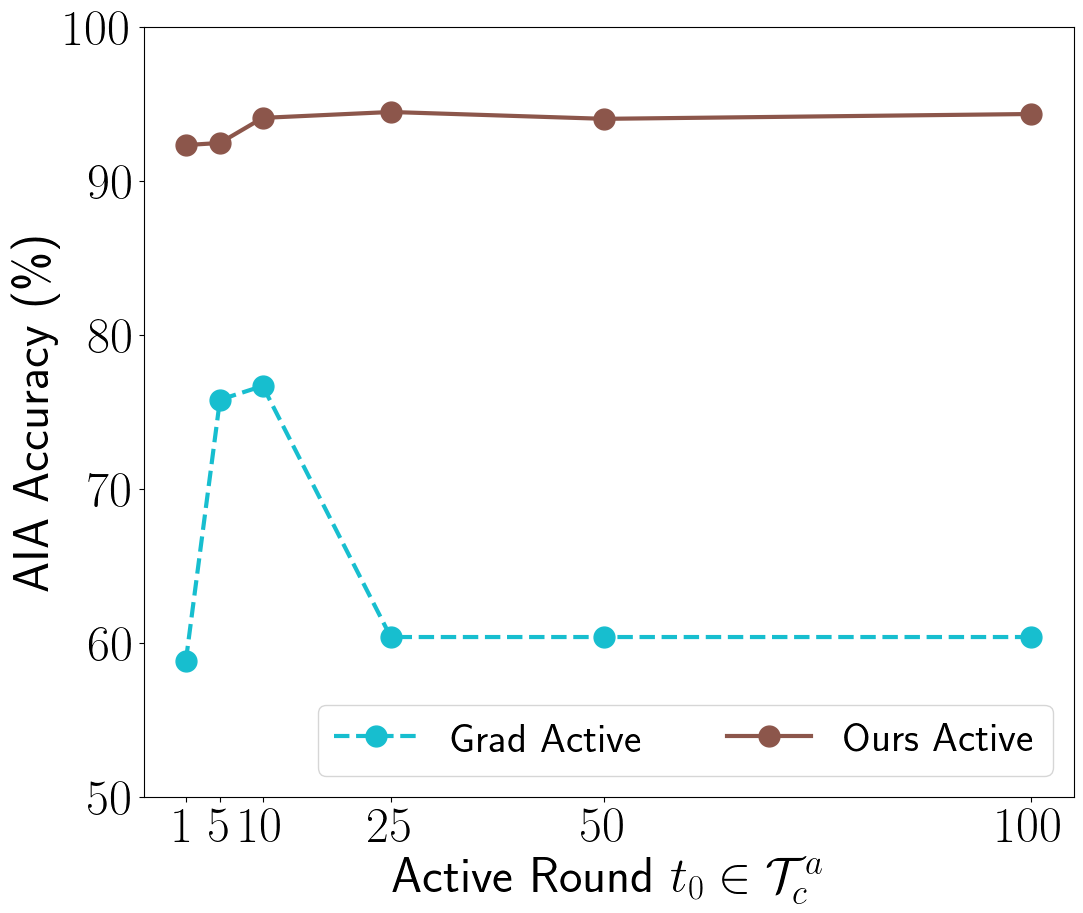
\includegraphics[scale=0.3]{assets/chapter_2/attack_round_effect.png}
    \caption{The AIA accuracy over all clients' local datasets under different starting points of active attack for Income-L dataset ($40\%$ heterogeneity level). The clients train a neural network through FedAvg with 1 local epoch and batch size 32.}
    \label{fig:attack_starting_point_effect}
\end{figure}


\subsection{Impact of the number of active rounds} 
\label{app:impact_active_rounds}
We evaluate the performance of active attacks under different numbers of active rounds $|\mathcal{T}^a_u|$ (Figure~\ref{fig:attack_round_effect}), during which an active adversary launches attacks.  Our attack becomes more powerful as the number of active rounds increases, whereas Grad does not demonstrate the same level of effectiveness.

\begin{figure}
    \centering
    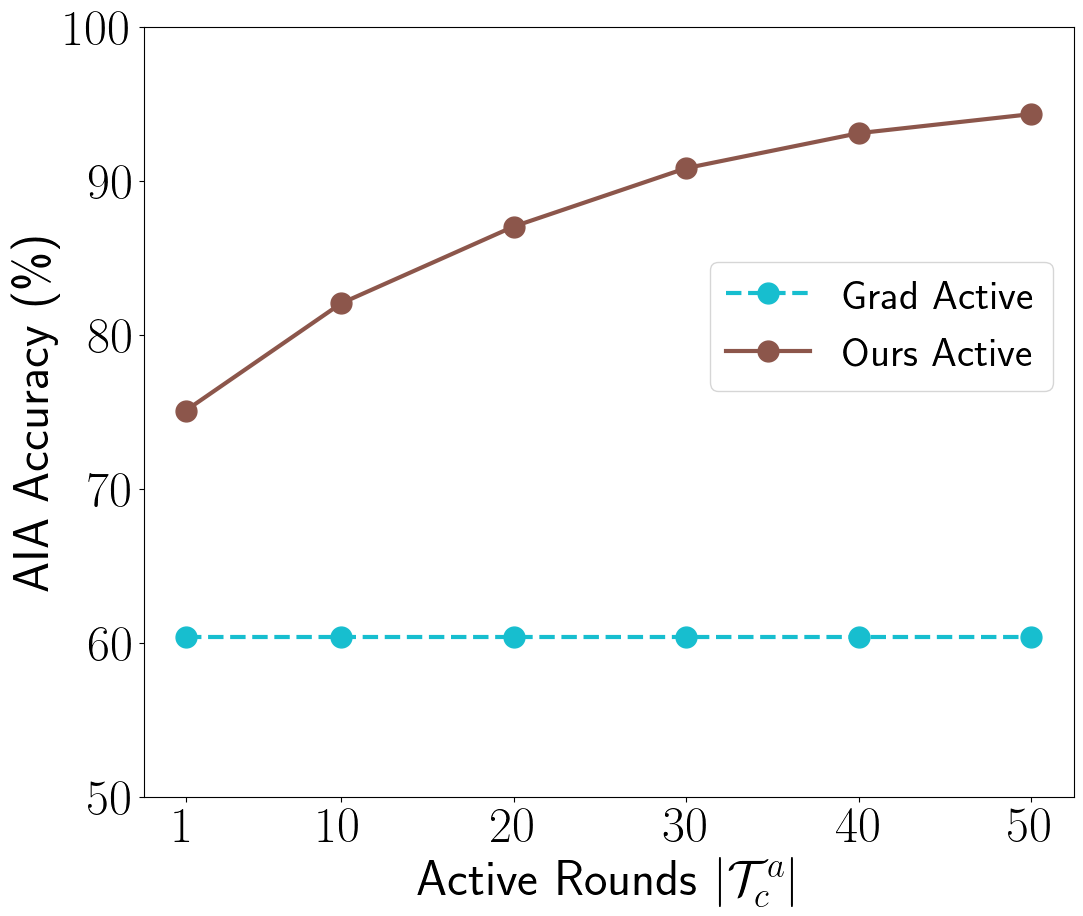
\includegraphics[scale=0.3]{assets/chapter_2/active_attack_traj_32_louisana.png}
    \caption{The AIA accuracy over all clients' local datasets under different numbers of active rounds for Income-L dataset ($40\%$ heterogeneity level). The clients train a neural network through FedAvg with 1 local epoch and batch size 32.}
    \label{fig:attack_round_effect}
\end{figure}



\subsection{Defense}
\label{app:defense}
To mitigate privacy leakage, we apply a federated version of DP-SGD~\cite{Abadi_dp}, which provides ($\epsilon, \delta$) sample-level differential privacy guarantees~\cite{Dwork, slDP}. More precisely, the clients clip and add Gaussian noises to their gradients in FL.  We used Opacus~\cite{Opacus} to incorporate a $(1,1\cdot10^{-5})$-differentially private defense on Income-L and Medical datasets, and $(1,1\cdot10^{-6})$-differentially private defense on Income-A.
All attacks are targeted at a randomly chosen single client. Other experimental settings are consistent with those used in the neural network experiments. 

\paragraph{Hyperparameters for defense}
We adjust the clipping norm for each dataset and select the one that yields the lowest validation loss in the final global model.
For Income-L and Income-A datasets, the clipping norm is tuned over the set $\{1\cdot 10^6, 3\cdot 10^6, 5 \cdot 10^6, 7\cdot 10^6, 9\cdot 10^6, 1\cdot 10^7, 3\cdot 10^7, 5 \cdot 10^7\}$. For Medical dataset, the clipping norm is tuned over the set $\{5 \cdot 10^5, 7\cdot 10^5, 9\cdot 10^5, 1\cdot 10^6, 3\cdot 10^6, 5 \cdot 10^6, 7\cdot 10^6, 9\cdot 10^6\}$.

%Clients train a neural network with a single hidden layer of 128 neurons using the ReLU activation function. The FedAvg protocol is employed with 1 local epoch, batch size 32 for 100 communication rounds.
%Hyperparameter tuning details for both training and attacks can be found in Appendix~\ref{app:hyperparameters}. 

\begin{table}[H]
    \centering
    \small
    \setlength{\tabcolsep}{6pt}
    \renewcommand{\arraystretch}{1.08}
    \begin{tabular}{@{}lccc@{}}
        \toprule
        \textbf{Attack} & \multicolumn{3}{c}{\textbf{Dataset}} \\
        \cmidrule(l){2-4}
        & \textbf{Income-L} & \textbf{Income-A} & \textbf{Medical} \\
        \midrule
        \multicolumn{4}{@{}l}{\textbf{Passive}} \\
        \quad Grad     & $59.34 \pm 3.58$          & $50.52 \pm 2.49$          & $63.51 \pm 6.63$ \\
        \quad Grad-w-O & $\mathbf{77.67} \pm 1.01$ & $53.83 \pm 0.19$          & $91.09 \pm 0.08$ \\
        \quad Ours     & $48.69 \pm 4.03$          & $\mathbf{58.08} \pm 0.11$ & $\mathbf{94.19} \pm 0.23$ \\
        \midrule
        \multicolumn{4}{@{}l}{\textbf{Active (10 rounds)}} \\
        \quad Grad     & $59.34 \pm 3.58$          & $50.52 \pm 2.49$          & $63.51 \pm 6.63$ \\
        \quad Grad-w-O & $\mathbf{77.67} \pm 1.01$ & $54.42 \pm 2.77$          & $91.09 \pm 0.08$ \\
        \quad Ours     & $62.04 \pm 3.16$          & $\mathbf{57.60} \pm 0.85$ & $\mathbf{93.96} \pm 0.41$ \\
        \midrule
        \multicolumn{4}{@{}l}{\textbf{Active (50 rounds)}} \\
        \quad Grad     & $59.34 \pm 3.58$          & $50.52 \pm 2.49$          & $63.51 \pm 6.63$ \\
        \quad Grad-w-O & $\mathbf{77.67} \pm 1.01$ & $54.42 \pm 2.77$          & $91.09 \pm 0.08$ \\
        \quad Ours     & $71.37 \pm 1.86$          & $\mathbf{57.25} \pm 0.86$ & $\mathbf{94.30} \pm 0.08$ \\
        \midrule
        Model-w-O      & $79.33 \pm 1.11$          & $58.53 \pm 0.61$          & $94.30 \pm 0.08$ \\
        \bottomrule
    \end{tabular}
    \caption{The AIA accuracy over one (random chosen) targeted client's local dataset evaluated under both honest-but-curious (passive) and malicious (active) adversaries across Income L, Income-A and Medical FL datasets. The standard deviation is evaluated over three FL training runs. All clients train a neural network through a federated version of DP-SGD with 1 local epoch and batch size 32, providing ($\epsilon=1$, $\delta=1\cdot 10^{-5}$) sample level differential privacy for every client on Medical and Income-L, and ($\epsilon=1$, $\delta=1\cdot 10^{-6}$) sample level differential privacy on Income-A.}
    \label{tab:dp_32}
\end{table}

Table~\ref{tab:dp_32} presents the results with both active and honest-but-curious adversaries. 
Our passive attacks significantly outperform Grad baselines on Income-A and Medical datasets, achieving over 30 and 8 percentage point improvements on Income-A and Medical datasets, respectively. Furthermore, our attacks improve also Grad-w-O baseline by 4 percentage points on Income-A and 3 percentage points on Medical. Surprisingly, passive gradient-based attacks demonstrate better performance than Ours on Income-L, despite having near-zero cosine similarity. This observation suggest that cosine similarity may not be a suitable metric for gradient-based attacks' optimization. Moving to the active adversary, our attacks exhibit minimal performance changes between rounds 10 and 50 on Income-A and Medical datasets, as they approach the empirical optimal performance achievable by Model-w-O. Conversely, on Income-L, where performance margins are larger, our attack surpass Grad by 3 and 12 percentage points after 10 and 50 active rounds, respectively, with potential for further optimization to match the optimal local model performance.
